\documentclass[../main.tex]{subfiles}
\renewcommand{\bm}[1]{\mathbf{#1}}

\begin{document}

\section{Lecture 1}{Inequalities and Sampling}

\begin{theorem}{Markov's Inequality}
    $\bb{P}(X \geq t) t \leq \bb{E}[X]$. Easy to see why. Note that this is only true
    for non-negative random variables.
    \label{thm:markov}
\end{theorem}

\begin{remark}
    This inequality is sharp, meaning that it cannot be further tightened. For example, let $X$ be a random variable that
    takes on $1$ with probability $1 - a$ and $0$ with probability $0$. Then $\bb{E}[X] = (1)(1 - a) + 0(a) \geq (1)(\bb{P}[X \geq 1]) = 1-a$. In this case, the $\geq$ is, in fact, an equality $=$.
\end{remark}

\begin{theorem}{Chebyshev's Inequality}
    It is UNRESOLVED why we need for $\text{Var}(X) < \infty$
    \[
        \bb{P}[(X - \bb{E}[X])^2 \geq t^2 \sigma_{x}^2] \leq \frac{1}{t^2}
    \]

    Note that this statement is also that

    \[
        \bb{P}[\abs{X - \bb{E}[X]} \geq t] = \bb{P}[(X - \bb{E}[X])^2 \geq t^2 ] \leq \frac{\sigma_x^2}{t^2}
    \]
\end{theorem}



\begin{proof}
    \begin{align*}
        \bb{P}(X \geq t) t &\leq \bb{E}[X]    \\
        \bb{P}(X^2 \geq t^2) t^2 &\leq \bb{E}[X^2]    \\
        \bb{P}((X - \mu_x)^2 \geq (t\sigma_x)^2) (t\sigma_x)^2 &\leq \bb{E}[(X - \mu_x)^2]    \\
        \bb{P}((X - \mu_x)^2 \geq (t\sigma_x)^2)  &\leq \frac{\bb{E}[(X - \mu_x)^2]}{(t\sigma_x)^2} = \frac{1}{t^2}    \\
    \end{align*}
\end{proof}

\section{Lecture 2}{Introduction to Randomization}
UNRESOLVED (MISSING MATRIX MULT AND TRIANGLES)

\begin{problem}{Expected Vertex Count}
    Suppose a graph has $n$ vertices and we randomly delete each vertex with probability $1/2$. The expected number of vertices is: \\

    Let $w$ be an array consisting only of $0$s and $1$s that is as long as there are vertices in $G$. Assume $w[x] = 1$ if the graph
    obtained from $G$ -- let us call it $H$ -- still has the $x$th vertex. It is easy to see that the probability of $H$ having those
    vertices denoted by $w$ is $\frac{1}{2^n}.$ Let $X(w)$ be the number of vertices that $H$ would have, were it represented by
    $w$. Let $X$ be the number of vertices $H$ has. \\
    
    Then $\bb{E}[X] = \sum_{w \in \Omega}^{} X(w) \frac{1}{2^n}$.  \\
    
    The right hand side of the inequality can be replaced by 
    $$\sum_{k=0}^{n} \underbrace{\text{ (The number of ways to get $k$ vertices multiplied by $k$ vertices) }}_{\alpha} \frac{1}{2^n}$$. Think about $\alpha$ for a second: for a given $k$ , $\alpha$ is really $\binom{n}{k} (k)$. \\

\end{problem}

\begin{problem}{Expected Edge Count}
    Suppose a graph has $n$ vertices and we randomly delete each vertex with probability $1/2$. The expected number of edges is: \\

    An edge $e$ is a connection between two vertices $u$ and $v$. Thus $e$ will continue to exist in $H$ if and only if $uv$ exists
    in $H$; that is, $u$ and $v$ must not be deleted, the probability of which is $1/4$. Let $E$ be the set of edges in $G$. Then
    the number of edges in $H$ is a random variable $X$ whose value is

    \[
        \sum_{(u,v) \in E}^{}X_[(u,v) \in E_H]
    \]

    where $X_{(u,v) \in E_H}$ is the binary random variable that takes on $1$ if $(u,v) \in E_H$ and $0$ otherwise. Its expectation is


    \[
        \sum_{(u,v) \in E}^{}\bb{P}[(u,v) \in E]
    \]

    which is just 

    \[
        \sum_{(u,v) \in E}^{}\frac{1}{4} = \frac{m}{4}
    \]
    
\end{problem}

\begin{outline}
    \1 Las Vegas algorithms are those algorithms that have a deterministic, correct ouput; however, these algorithms have a random running time depending on the input they're supplied with.
    \2 We are commonly interested in bounding their worst case expected running time. This quantity can be called $T(n)$, and it can be expressed as: 

    \[
        T(n) = \max_{X: \abs{X} = n} \bb{E}[X] \tag{$\alpha$}
    \]

    \1 Monte Carlo algorithms have a random output but a deterministic running time. We want to calculate what is the minimum probability that the algorithm produces an accurate output.
    \2 This can be expressed as 

    \[
        T(n) = \min_{X : \abs{X} = n } \bb{P}[f(X) \text{ ``is correct" }]
    \]
\end{outline}

\breathe \\
I now present two ways to analyze randomized quick sort. Recall that quick sort chooses a pivot in an array, sorts all elements in the array according to the pivot, and then recursively sorts the
``sorted'' halves. Let $Q(A)$ be the number of comparisons made
in order to quick sort $A$. Suppose $A_n$ has $n$ elements; then

\[
    Q(A_n) = \sum_{i=1}^{n} X_{i}\left( ( [Q(A_{i-1})] + [Q(A_{n-i})] \right)
\]

where $X_{i} = 1$ if $i$ is a pivot and $0$ otherwise.

\[
    Q(A_n) = \sum_{i=1}^{n} X_{i}\left( ( [Q(A_{i-1})] + [Q(A_{n-i})] \right)
\]

Now apply expectation to get:

\[
    \bb{E}[Q(A_n)] = \sum_{i=1}^{n}\bb{E}[X_{i}]\left( \bb{E}[Q(A_{i-1})] + \bb{E}[Q(A_{n-i})] \right) + n
\]

We skipped a step in that we jumped from $\bb{E}[Q(A_{j})X_{j+1}]$ to $\bb{E}[Q(A_{j})] \bb{E}[X_{j+1}]$. This is justified because $Q(A_{j})$ is independent of $X_{j+1}$; for the coin flips\footnote{We use coinflips to simulate a uniform distribution} used to choose pivot $j+1$ are independent of the coin flips that will be used in $A_{j}$.

\[
    \bb{E}[Q(A_n)] = \sum_{i=1}^{n}\frac{1}{n}\left( \bb{E}[Q(A_{i-1})] + \bb{E}[Q(A_{n-i})] \right) + n \tag{$\beta$}
\]


This recurrence is true for all inputs $A$ of size $n$ and, in particular, for the input that would require the maximum running time. Thus, if we define $T(n)$ as we did in $(\alpha)$, then the expression above becomes

\[
    T(n) \leq n + \sum_{i=1}^{n}\frac{1}{n}\left( T(i-1) + T(n-i) \right)
\]

Notice that we replaced $=$ with $\leq$, for the use of $T(n)$ means that we are working with maximums, and so the inequality in $\beta$ becomes less tight. For first (UNRESOLVED).

At this point, we can (UNRESOLVED) verify that this run time follows $O(n \log n)$ by running an inductive proof.

Another approach is to define $R_{ij}$ as the event that the $i$th rank element is compared with the $j$th rank element and to define $X_{ij}$ as the associated binary random variable. Thus, the total number of comparisons (and, hence, the running time of randomized quick sort) is given by 

\[
    X = \sum_{1 \leq i < j \leq n }^{}X_{ij}
\]

where $X$ is the total number of comparisons; whence

\[
    \bb{E}[X] = \sum_{1 \leq i < j \leq n }^{}\bb{E}[X_{ij}]
\]


\[
    \bb{E}[X] = \sum_{1 \leq i < j \leq n }^{}\bb{P}[R_{ij}]
\]

\begin{lemma}
    $\bb{P}[R_{ij}]$ is $\frac{2}{j-i+1}$.
\end{lemma}

\begin{proof}
    Identifying the $i$th through $j$th ranked elements as $\{i \dots j\}$, observe that $i$ is compared with $j$ if and only if the pivot chosen from among $\{i \dots j\}$ is either $i$ or $j$. Since pivot selection happens uniformly at random, there are two desireable values to choose from and $j - i + 1$ total values, the probability of $R_{ij}$ is as stated.
\end{proof}

Whence

\begin{align*}
    \bb{E}[X] &= \sum_{i=1}^{n-1}\sum_{j=i+1}^{n}\frac{2}{j-i+1} \\
    &= \sum_{i=1}^{n-1}\sum_{\delta=2}^{n-i+1}\frac{2}{\delta} \\
    &= 2 \left(\sum_{i=1}^{n-1} H_{n-i+1} - 1\right)  \\
    &\leq  2 \left(\sum_{i=1}^{n-1} H_{n-i+1} \right)  \\
    &\leq  2 \left(\sum_{i=1}^{n-1} \log n \right)  \\
    &\leq  2 n \log n  \\
\end{align*}

Note that

\[
    \sum_{x=1}^{n}\frac{1}{x+1} \leq \underbrace{\int_{1}^{n}\left( \frac{1}{x} \right)}_{\ln(n)} \leq \sum_{x=1}^{n}\frac{1}{x}
\]

which establishes that $H(n) = \Theta(n)$, since both the left hand side and the right hand since


\[
    H_n = O(\sum_{x=1}^{n}\frac{1}{x+1}) \leq \underbrace{\int_{1}^{n}\left( \frac{1}{x} \right)}_{\ln(n)} \leq O(\sum_{x=1}^{n}\frac{1}{x}) = H_n
\]

\section{Lecture 3}{Probabilistic Inequalities}

\begin{remark}
    If we toss a fair coin $n$ times then the probability of getting $k$ heads is

    \[
        \binom{n}{k}(1/2^n)
    \]

    Recall that this holds, because any one sequence of heads and tails has a $\frac{1}{2^n}$
    probability of taking place; finally, there are $\binom{n}{k}$ such sequences that
    have $k$ heads.
\end{remark}

\begin{remark}
    Suppose we know that a random variable $Q$ satisfies $\bb{P}[Q \geq 10 n \log n] \leq c$. And we know that $Q \leq n^2$. Argue that $\bb{E}[Q] \leq 10 n \log n + (n^2 - 10 n \log n)c$.

    \begin{align*}
        \intertext{First note that} \\
        \bb{P}[Q < 10 n \log n] > 1 - c \\
        \intertext{It, therefore, follows that:} \\
        \bb{E}[Q] \leq n^2 \times (\bb{P}[Q \geq 10 n \log n]) + (\bb{P}[Q < 10 n \log n])(10 n \log n) \\
        = \bb{E}[Q] \leq n^2 \times (c) + (1 - c)(10 n \log n) \\
    \end{align*}

    This gives us what we desire.
\end{remark}

\begin{remark}
    Recall that if $X$ and $Y$ are independent, then $\text{Var}(X + Y) = \text{Var}(X) + \text{Vary}(Y)$ and that $\bb{E}[XY] = \bb{E}[X] \bb{E}[Y]$.
\end{remark}

\begin{remark}
    The Chebyshev bound is not, in certain cases, strong enough: \\

    Suppose that we simulate a one dimensional random walk; a random variable $X_{i}$
    takes on $-1$ at time $i$ if we move left at time $i$ and otherwise takes the value
    $1$. We wish to put bounds on the variable $Y = \sum_{i=1}^{n}X_{i}$. \\

    Observe that $\bb{E}[Y] = \sum_{i=1}^{n}\bb{E}[X_{i}] = 0$ and that, since all the
    $X_{i}$ are independent, 

    \[
        \var{Y} = \sum_{i=1}^{n} \var{X} = \sum_{i=1}^{n}\Ex{X^2} - \Ex{X}^2 \sum_{i=1}^{n}(1) = n
    \]

    Because of this, we can use Chebyshev's inequality. 

    \begin{align*}
        \prob{\abs{Y - \Ex{Y}} \geq t} \leq \frac{\sigma_x^2}{t^2} \\
        \prob{\abs{Y - \Ex{Y}} \geq t\sqrt{n}} \leq \frac{n}{nt^2} = \frac{1}{t^2} \\
        \prob{\abs{Y} \geq t\sqrt{n}} \leq \frac{n}{nt^2} = \frac{1}{t^2} \\
    \end{align*}
\end{remark}

\begin{center}
    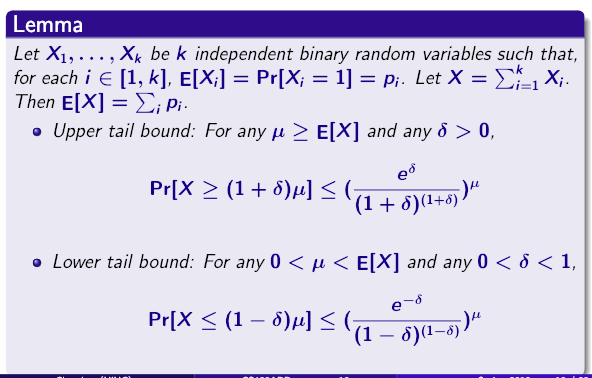
\includegraphics[width=\textwidth,height=\textheight,keepaspectratio]{lecture3_chernoff_nonneg}
\end{center}

\begin{remark}
    The chernoff bound given before can be simpliefied in the case that $0 < \delta < 1$:

\begin{center}
    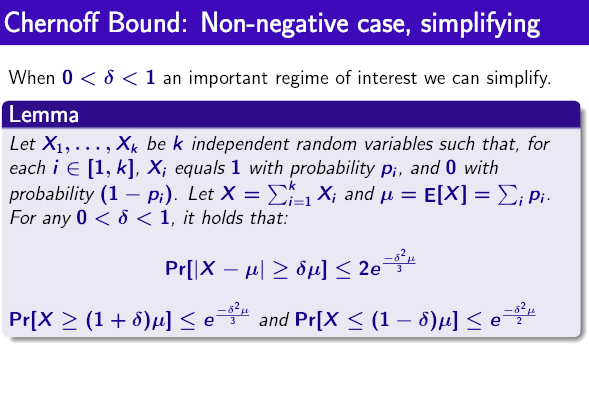
\includegraphics[width=\textwidth,height=\textheight,keepaspectratio]{lecture3_chernoff_nonneg_simp}
\end{center}

\end{remark}

\begin{remark}
    If we allow the random variables to take on negative values as well, then we find that
    the new bound depends on the number of variables (the dimension), whereas the theorem
    involving non-negative random variables was dimension free.

    \begin{center}
        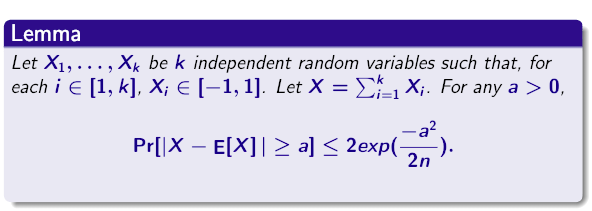
\includegraphics[width=\textwidth,height=\textheight,keepaspectratio]{lecture3_chernoff_general}
    \end{center}


    Applying this new finding to the random walk example presened earlier, we see that
    we can revise the bounds to be

    \begin{align*}
        \prob{\abs{Y} \geq t\sqrt{n}} \leq 2 \exp{-t^2/2} = \frac{1}{t^2} \\
    \end{align*}

\end{remark}


\begin{example}
    Suppose that we toss $n$ balls into $n$ bins (or consider that we toss $m$ balls into $n$ bins). We wish to bound the random variable $Y$, which we set to the maximum number of balls in any bin. To do so, we employ the following procedure:

    \begin{outline}
        \1 Focus on one bin, and bound the probability that this one bin receives more than a certain number of balls.
        \2 Express this probability by first defining binary random variables that represent the probability that a ball falls into this chosen bin.
        \2 Use the chernoff bounds to define a bound (when we work forward, we will usually have to leave this bound expressed as a variable; at the end of the exercise, it will be clear what bound to set.
        \1 Apply the union bound to bound the probability that all bins receive more than a certain number of balls.
        \2 Use this to define the maximum number of balls that fall into any one bin.
        \1 Compute the expectation in a manner similar to the example shown earlier.
    \end{outline}

    Let $X_{ij}$ be the event that ball $j$ falls into bin $i$. Then set 

    \[
        X_{i} = \sum_{i=1}^{n}X_{ij}
    \]

    where $X_{i}$ represents the number of balls that fall into bin $i$. One Chernoff bound tells us that for $\delta > 0$, we have

    \[
        \prob{\abs{X_{i} > (1 + \delta)\mu }} \leq (\frac{e^{\delta}}{(1 + \delta)^{1 + \delta}})^{\mu}
    \]

    In this case note that $\Ex{X_{i}} = \sum_{i=1}^{n}1 /n = 1$. \\

    Whence, this simplifies to.
    \[
        \prob{\abs{X_{i} > (1 + \delta) }} \leq (\frac{e^{\delta}}{(1 + \delta)^{1 + \delta}})
    \]

    For a second (ie, we will be concrete about this later by choosing a suitable values for $\delta$), assume that

    \[
        (\frac{e^{\delta}}{(1 + \delta)^{1 + \delta}})^{\mu} < \frac{1}{n^3}
    \]

    Now observe that if we let $A_{i}$ be the event that $X_{i} > (1 + \delta)$

    \[
        \prob{\un_{i=1}^{n}A_{i}} \leq \sum_{i=1}^{n}\prob{A_{i}} = 1/n^2
    \]

    Then the probability that the maximum of any bin $Y$ is less than $(1 + \delta)$ is precisely the probability that that all bins have less than $(1 + \delta)$. This is at least $1 - 1/n^2$. Whence, we can say, \textit{with high probability} that this works. \\

    Given that $Y \leq n$, we can bound $\Ex{Y}$ by

    \[
        (1 - 1/n^2)(1 + \delta) + 1/n^2(n)
    \]

    UNRESOLVED: It is not known how the quantity:

    \[
        \left( \frac{e^{\delta}}{(1 + \delta)^{(1 + \delta)}} \right)^{\mu}
    \]

    can be massaged into $\frac{1}{n^3}$.
\end{example}

\begin{remark}
    Recall that the variance of a binary random variable is $p^2 - p = pq$ since $\Ex{ X }^2 - \Ex{ X }^2$.
    
    The notes leave open the question of, assuming that
    a single ball first (before all other balls) falls into bin $j$, then what is the expected number of balls
    that will fall into $j$ afterwards, what is the variance of this quantity and can we give a high probability bound (the answer to the latter being: yes, use the chernoff bound where the LHS is $\prob{X \leq (1 + \delta) \mu}$.
\end{remark}


\begin{example}{$\e$ representative Median Array}
    \begin{problem}
        We wish to devise an algorithm such that given a list $A$ we can choose an element $x$ such that the rank of $x$ is 

        \[
            (1 - \e)n/2 \leq \text{rank}(x) \leq (1 + \e)n/2
        \]

        Devise a randomized algorithm for this that outputs a desireable element with high probability
    \end{problem}
    \begin{solution}
        Sample from the array $k$ times with replacement. Output the median of the sample. This works:
        
        
        Set $S$ to be the set obtained. Set $M$ to be 
        \[
            \{ y | (1 - \e)n/2 \leq \text{rank}(y) \leq (1 + \e)n/2\},
        \]
        $L$ to be the left portion of $A$ and $R$ to be right portion of $A$. Observe that if this algorithm does not produce a desireable candidate, then necessarily either

        \[
            \abs{S \cap L} \geq k/2 \text{ or } \abs{S \cap R} \geq k/2\footnote{For if this were not the case, then $\abs{S \cap M} $ would not be non empty.}
        \]

        The more helpful observation is that if both 
        \[
            \abs{S \cap L} < k/2 \text{ and } \abs{S \cap R} < k/2
        \]

        then, the algorithm does produce a good solution.


        WOLOG, let us make a probability bound that $\abs{S \cap L} < k/2$.

        Using the (UNRESOLVED) first cherner inequality, we can show that for a sufficiently large value of $k$, we have 
        \[
            \prob{\abs{S \cap L} \geq k/2} < \delta/2
        \]

        Running the same argument, we find that

        \[
            \prob{\abs{S \cap R} \geq k/2} < \delta/2
        \]

        whence

        \[
            \prob{\text{That either of the preceding two events take place}} \leq \sum_{}^{}\prob{\text{That either of the two events take place alone}} = \delta
        \]

        It follows that neither event will take place with probability $1 - \delta$.

    \end{solution}
    
    We outline the strategy of the approach (UNRESOLVED)
    \begin{outline}
        \1 Realize that
    \end{outline}
\end{example}

\begin{example}
    We established that randomized quick sort takes $O(n \log n)$ time in expectation and, otherwise, require $O(n^2)$ time. We wish to concretely bound

    \[
        \prob{Q > n \log n}
    \]

    where $Q$ is the number of comparisons that quick sort makes.

    Our strategy is as follows:
    \begin{outline}
        \1 Observe that if $k$ levels of recursion take place then $Q \leq kn$.\footnote{We call $k$ the depth of the recursion.} 
        \2 Whence it suffices to show that $k \leq \text{some constant} \times \log n$.
        \1 We will make a bound on the depth of recursion by proving that, with high probability, the number of levels of recursion involving any one element is bounded by $\text{some constant} \times \log n$.
        \1 Applying the union bound, we will conclude that the total depth of recursion is less than some constant multiplied by $\log n$ with high probability.
    \end{outline}

    Fixing an element $s \in A$, we let $S_{i}$ be the partition of $A$ that contains $s$ on the $i$th iteration of quick sort. Call an iteration $i$ lucky if $\abs{S_{i+1}} \leq \frac{3}{4}\abs{S_{i}}$ and if $\abs{S_{i+1} \smallsetminus S_{i}} \leq \frac{3}{4}\abs{S_{i}}$. The probability that any one iteration is lucky is independent of the probability that a subsequent or later iteration is lucky, and the probability that an interation is lucky is $\frac{1}{2}$. UNRESOLVED :It is not presently known why we care that $\abs{S_{i+1} \smallsetminus S_{i}} \leq \frac{3}{4}\abs{S_{i}}$. We observe that
    
    if we let $\rho$ be the number of lucky iterations, desire that $\abs{S_{k}} = 1$, and use the fact that

    \[
        \abs{S_{k}} \leq (3/4)^\rho n
    \]

    then $(3/4)^\rho n = 1 \implies \rho \ln(3/4) = \ln(1/n) \implies \rho = \frac{\ln(n)}{\ln(4/3)} = \log_{4/3} n \leq 4 \ln(n)$. We will show that within $k = M \log n$ iterations for some $M > 0$, at least $4 \ln (n)$ lucky iterations take place (with high probability) for each member of $A$. This will allow us, with high probability, to bound the probability that all members of $A$ have $4 \ln (n)$ lucky iterations within $M \log(n)$ iterations.

    Let $X_{i}$ be a binary random variable that is $1$ if the $i$th iteration is lucky and $0$ otherwise. Observe that
    $\Ex[X_{i}] = 1/2$ (convince yourself). Thus the expectation is $k/2$. We can then use Chernoff to make a bound:

    \[
        \text{Set $k = 32 \ln n$ and $\delta = 3/4$} \\
        \prob{\rho \leq 4\ln n} = \prob{\rho \leq \mu(1 - \delta)} \\
    \]


    \begin{center}
        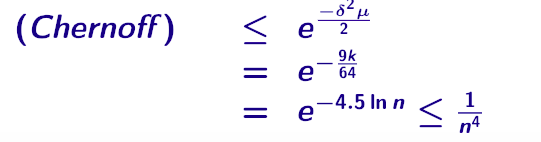
\includegraphics[width=\textwidth,height=\textheight,keepaspectratio]{lecture3_final_randomized}
    \end{center}

    The probability that any on element has the preceding fate befall them is $1/n^3$. Thus, with probability $1 - 1/n^3$, no element will have this fate befall them, and the algorithm will end after $32 \ln n$ comparisons. UNRESOLVED (again, it is not known how we could have derived the bounds that we set earlier.
\end{example}




\section{Lecture 4}{$i$-wise Independence and Hashing}
\begin{remark}
    It is expensive to store $n$ random bits. We need a way to obtain $n$ random variables
    without paying for the price to store $n$ random variables.
\end{remark}

\begin{definition}
    Givey random variables $Y_1 \dots Y_k$ with range $[B]$, we say that the random variables
    are totally independent if 

    \[
        \prob{\{Y_i = b_i\} \forall i} = \prod_{i} \prob{Y_{i} = b_{i}}
    \]
\end{definition}

\begin{lemma}
    It is easy to check that if a set of totally random variables is totally random in
    any of its subsets.
\end{lemma}

\begin{example}
    A set of pairwise random variables is not necessarily totally independent.

    Suppose that $X_1$ and $X_2$ are independent. Let $X_3 = f(X_1, X_2)$ where
    $f$ is some deterministic function THen $X_3$ is not independent with
    $X_1$ and $X_2$, since knowing the latter two implies knowing the former.
\end{example}

\begin{theorem}
    Index $k$ uniformly random bits by $[k]$ so that $X_{i}$ is the random variable 
    whose value is the value of bit $i$. Let $T$ be a subset of $[k]$ an let
    $S_{T} = \oplus_{T} X_{i}$. Then if $T \not = Q$, we have that $T$ and $Q$ are independent.
\end{theorem}

\begin{proof}
    Sketch: Consider $T \cap Q = \emptyset$, $T \s Q$ and $T \cap Q \not = \emptyset$ but $T \not \s Q$. In each case, let $v_{TQ}$ be the value obtained by taking the $\oplus$ of indices common to $T$ and $Q$. There is at least one index that $T$ and $Q$ differ by, call it $s$ and assume without loss of generality that $T$ has it. Then $Y = v_{TQ} \otimes X_s$ is a uniformly random bit, since it takes on $1$ as often as it takes on $0$; it is independent of $v_{TQ}$ since $v_{TQ}$ does not influence $Y$ to be anything other than uniformly distributed. If $T$ and $Q$ differ by any other bits, then we can apply the foregoing analysis to $Y$ and $Q$.
\end{proof}

\begin{theorem}
    Given $\log n$ random bits, we can construct $n$ random bits\footnote{Whenever we speak of random bits, we will implicitly assume that they are randomly distributed.} on the fly. 
\end{theorem}

\begin{proof}
    Apply the preceding theorem. Notice that we only have to store $\log n$ bits as opposed to $n$.
\end{proof}

\begin{remark}
    If we want to make $n$ random variables that are each uniformly distributed in $\{1 \dots k\}$, then convince yourself that we need $\log n \log k$ random bits. To see this imagine that we have laid out $\log m$ cubbies. When each of these $\log m$ cubbies takes a value, we will get a number in $\{1 \dots k\}$. In order to get $n$ such random numbers, it suffices that each of these cubbies have $n$ different random functions that fill these cubbies. We need $\log n$ bits to do that. Thus, each cubby is fillable by the function obtained by taking the $\oplus$ of some subset of these $\log n$ bits. This is why we need $\log n \log k$ bits. 
\end{remark}

\begin{remark}
    Always imagine in these scenarios that we want to construct some
    random variables from random bits (and not just random values). That is, using some small number of random bits, we want to be able to create independent random functions that we pass on to some application. These functions can share parts, but these must ultimately themselves be random. Also helpful is to remember that these functions will take on random values, each time you provide them with random inputs. That is, pretend that you shake out random bits from a cup, and then insert those bits into random functions.
\end{remark}

\begin{lemma}
    If $x \in \ZZ_{p}$ where $p$ is prime then there is a unique $y \in \ZZ_{p}$ such that $xy = 1 \mod p$. The proof is on his notes around page 13.
\end{lemma}

\begin{remark}
    As a consequence, $\ZZ_{p}$ is a field, and it admits division.
\end{remark}

\begin{lemma}
    If $x \not = y$ and $(r,s) \in \ZZ_p \times \ZZ_p$, there is equality one pair $(a,b) \in \ZZ_p \times \ZZ_p$ such that

    \[
        ax + b = r \text{ and } ay + b = s
    \]

\end{lemma}

\begin{proof}
    Solve for $a$ and $b$ using this equation:

    \[
        ax + b = r \text{ and } ay + b = s
    \]

    We have $b = r - ax$ and $a = \frac{r - s}{x - y}$.

    This tells us that if we know $(a,b)$ then we know $(r,s)$ and
    vice versa.
\end{proof}

\begin{theorem}
    We can create $p$ random variables with range $[p]$ using
    only $2 \lceil \log p \rceil$ random variables.
\end{theorem}

\begin{proof}
    Twice, using $\log p$ bits each time, get a value in $[p]$. Define $X_{i} = ai + b \forall i \in [p]$. \\

    Observe firstly that each $X_{i}$ is uniformly distributed. That is, for each $y \in [p]$, we have $\abs{\inv{X_{i}}(y)} = p$. This is easy to verify, since whatever the value of $ai$, as $b$ varies over $[p]$ $ai + b$ will take on all values. \\

    Now we claim that $X_{i}$ and $X_{j}$ are pairwise independent for $i \not = j$. We need to show that:

    \[
        \prob{X_{i} = m \text{ and } X_{j} = n} = \prob{X_{i} = m}\prob{X_{j} = m} = 1/p^2
    \]

    From the previous theorem, we know that given a pair $(m,n) \in \ZZ_p \times \ZZ_p$, the pair $(a,b)$ that satisfies the foregoing equations is unique. The probability that this unique pair is chosen is $\frac{1}{p^2}$ and, thus, we are done.
\end{proof}

\begin{remark}
    Note that the claim that independent $\{X_{i}\}_{i \in [n]}$ where $X = \sum_{i=1}^{n}X_{i}$ satisfy

    \[
        \var{X} = \sum_{i=1}^{n}\var{X_{i}}
    \]

    is sufficient if the $X_{i}$ are pairwise independent.
\end{remark}

\begin{proposition}
    If we want to construction $n$ pairwise independent random variables that have range $[m]$, where $n \not = m$, the previous construction involving $p$ random variables that have $[p]$ range can be modified.
\end{proposition}

\begin{proof}
    Assume first that $n < m$:

    There is always a prime $p \in [m, 2m]$. Using this $p$, invoke
    the previous construction but take only $n$ random variables 
    instead of all $p$.

    Assume now that $n > m$. 

    \begin{lemma}
        All finite fields are of the form $p^k$ where $p$ is prime $k \geq 1$. Given any prime $p$ and $k \geq 1$, there is a field of order $p^k$ that is unique up to isomorphism.
    \end{lemma}

    If we use this lemma, then we can at least provide a construction
    for when $n$ and $m$ are powers of $2$. Invoke the construction
    using $n$. Now take the $n$ resultant random variables and truncate them by removing their first $\log m - \log n$ bits. This will leave
    them in the range $[m]$. These random variables are still
    uniformly distributed (for every power $k$ of $2$ where $k > m$, all possible arrangements of bits occurring in $X_{i}[0:m-1]$ will appear twice more), so no one arrangement is skewed. The random variables are still pairwise independent: $X_{i}$ and $X_{j}$. Sketch: When the first $\log n - \log m$ bits existed, there was a unique $(a,b)$ that allowed $X_{i} = x$ and $X_{j} = y$. Now there are $2n/m = 2^{1 + \log n - \log m}$ copies; the probability is thus $2n/m \bigg/ n^2$ that an acceptable of $(a,b)$ is chosen. The probabiliy that $X_{i} = x$ or that $X_{j} = y$ is $2n/m = 2^{1 + \log n - \log m}$.
\end{proof}


\begin{definition}
    Suppose a family $\mc{H}$ of hash functions is given. Then
    $\mc{H}$ is 2-strongly universal if, for any distinct $x,y$ and $h \in \mc{H}$ chosen uniformly at random, it holds that
    $h(x)$ and $h(y)$ are independent. Moreover, fixing $x$
    and letting $h$ vary, $h(x)$ is uniformly distributed.
\end{definition}

\begin{definition}
    $\mc{H}$ is 2-universal if for all distinct $x,y$ it holds
    that $x\prob{h(x) = h(y)}_{h \in \mc{H}} \leq \frac{1}{n}$.
\end{definition}

\section{Lecture 5}{More on Hashing and Morris's Algorithm}
\begin{theorem}
    Assuming that we use separate chaining (ie when a collission takes place at some bucket, just append to a linked list at that bucket to add the element that resulted in the collission), then if we hash $n = \abs{S}$ elements to a table of size $m = \abs{T}$, assuming that we also choose a hash function uniformly at random from a universal hash family, the probability that a collision takes place is $n/m$,
\end{theorem}
\begin{proof}
    Let $l(x) = T(h(x))$ be the size of the linked list at the bucket at the bucket mapped to by $x$. We wish to calculate
    $\Ex{l(x)}$. For any other $y$, let $D_y$ be the binary random variable representing the event that $y$ maps to $x$. Then

    \begin{align*}
        \Ex{l(x)} = \sum_{y \in S}^{}\Ex{D_{y}} \\
         = \sum_{y \in S}^{}\prob{h(x) = h(y)}.
         \leq \sum_{y \in S}^{}\frac{1}{m}.
    \end{align*}

    Since $\mc{H}$ is universal, the probability that $h(x)
    = h(y)$ is at most $1/m$.
\end{proof}

\begin{theorem}
    Assume that $N =\abs{\mc{U}}, m = \abs{T}, n = \abs{S}$. Let $p \geq N$ be prime. Let $a,b \in [p]$. Then the set of hash functions given by
    $\mc{H} = \left\{h_{a,b}| h_{a,b} = ax + b \mod p \mod m  \right\}$ is universal.
\end{theorem}

\begin{proof}
    First observe that the probability of a bucket being chosen is not exactly uniformly distributed. While $h_{a,b}$ restricted to $\mod p$ is uniformly distributed, where $a$ and $b$ are chosen uniformly at random, $h_{a,b}$ fails to be truly uniformly random because it involves an outer $\mod$ under $m$. This outer $\mod$ suggests that some buckets (bear in mind that
    the regime $p > m$ is at work) -- in particular some of the buckets $p \mod m$ buckets that are left over -- will be filled while the $m - p \mod m$ buckets will not be. In fact the probability that the $p \mod m$ buckets will be chosen -- and, thus, the greatest probability that a bucket can be chosen -- is

    \[
        \frac{\lfloor p/m \rfloor + 1}{p} \leq \frac{\lceil p/m \rceil}{\floor p/m \rfloor m} 
    \]


    In class, it was claimed that this function does have a collission probability of less than $1/m$, however. UNRESOLVED -- they seem to claim that if $x \not = y$ then $ax \not = ay \mod p$ without requiring that $x \not = y \mod p$; then they argue that adding $b \mod p$ to the expression $ax$ or $ay$ will have the collission be less than $1/m$.
\end{proof}

\begin{definition}
    A bloom filter is a collection $\mc{H}$ of hashing functions that records whether an object was seen or not. Given an input $x$ and $h \in \mc{H}$, we mark the bucket $h(x)$ by $1$. When we are given an element $y$, we claim that $h(y)$ exists if $h(y) = 1$ and otherwise claim it does not exist. We do this for each $h \in \mc{H}$. Let the false probability of $y$ existing be $\alpha$ for any $h \in \mc{H}$ be $\alpha$. The bloom filter claims that an element exists iff all $h \in \mc{H}$ map that element to $1$. Thus the probability of error is $\alpha^{\abs{\mc{H}}}$.
\end{definition}


\begin{remark}
    We need $\log n$ bits to deterministically count to $n$. What if we kept track of $\log n$, however? Well, there is no function in place to calculate $\log n$ (at least not cheaply) -- so we will keep track of $\log n$ using a randomized algorithm. In expectation, it will turn out that this algorithm gives us the right answer.
\end{remark}

\begin{definition}{Morris's Counting Algorithm}

    \begin{algo}
        X \leftarrow 0 \\
        while objects come in: \+\\
        Flip a coin with probability $\frac{1}{2^{X}}$.
        If heads: \+\\
        X \leftarrow 0 \-\-\\
        Return $2^{X} - 1$ \\
    \end{algo}
    
\end{definition}
\begin{proof}
    The proof proving that this works in expectation is
    given in Chekuri's Lecture 5 notes.
\end{proof}

\begin{remark}
    Chekuri also shows that the variance of this algorithm is $O(n^2)$.
\end{remark}<++>

\begin{remark}
    If we can provide an expectation and variance for an algorithm's running time, then observe that if we operate that algorithm $n$ times independently (or, perhaps, in parallel), and take the average of the algorithms' results, then the variance of the resulting algorithm's accuracy drops by a factor $1/n$.
\end{remark}


\end{document}



